
\documentclass[border=8pt, multi, tikz]{standalone} 
\usepackage{import}
\subimport{../../../tools/PlotNeuralNet/layers/}{init}
\usetikzlibrary{positioning}
\usetikzlibrary{3d} %for including external image 

\usetikzlibrary{calc,decorations.pathreplacing,fit}
\def\IOColor{rgb:white,4;black,1}
\def\ConvColor{rgb:yellow,5;red,2.5;white,5}
\def\ActColor{rgb:yellow,5;red,5;white,5}
\def\PoolColor{rgb:red,1;black,0.3}
\def\UpColor{rgb:blue,2;green,1;black,0.3}
\def\CopyColor{rgb:white,1;black,3}
\def\OutColor{rgb:magenta,5;black,7}
\def\GraphColor{rgb:blue,5;green,2.5;white,5}
\def\GraphActColor{rgb:blue,5;green,5;white,3}
\def\SumColor{rgb:blue,5;green,15}
\def\DCColor{rgb:red,2;blue,5;white,2}
\def\HLCCColor{rgb:green,3;blue,1;white,8}

\newcommand{\copymidarrow}{\tikz \draw[-Stealth,line width=0.8mm,draw={rgb:blue,4;red,1;green,1;black,3}] (-0.3,0) -- ++(0.3,0);}

\begin{document}
\begin{tikzpicture}
\tikzstyle{connection}=[ultra thick,every node/.style={sloped,allow upside down},draw=\edgecolor,opacity=0.7]
\tikzstyle{copyconnection}=[ultra thick,every node/.style={sloped,allow upside down},draw={rgb:blue,4;red,1;green,1;black,3},opacity=0.7]

\tikzstyle{bus}=[ultra thick,-Stealth,draw={rgb:blue,4;red,1;green,1;black,3},opacity=0.7,rounded corners=4pt]
\tikzstyle{op}=[draw=black!60,fill=\HLCCColor,rounded corners=3pt,align=flush center,font=\small,inner sep=4pt]

\pic[shift={(0,0,0)}] at (0,0,0)
    {Box={name=in,
        caption={},
        xlabel={{"",}},
        zlabel={},
        fill=\IOColor,
        opacity=0.6,
        height=24.0,
        width=0.4,
        depth=17.1}};

\begin{scope}[shift={(in-east)}]
    \node[canvas is zy plane at x=0,transform shape,inner sep=0pt] at (0,0)
        {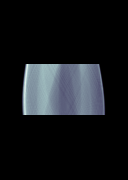
\includegraphics[width=3.420cm,height=4.800cm]{sinograms/incomplete.png}};
\end{scope}

\node[below=12pt,align=center,font=\small] at (in-nearsoutheast) {\textbf{Incomplete $y$}\\$180\times128$};

\pic[shift={(2.0,0,0)}] at (in-east)
    {RightBandedBox={name=menc0,
        caption={},
        xlabel={{"","",}},
        zlabel={},
        fill=\ConvColor,
        bandfill=\ActColor,
        opacity=0.4,
        height=24.0,
        width={0.6,0.6},
        depth=16.7}};

\draw [connection]  (in-east)    -- node {\midarrow} (menc0-west);

\pic[shift={(0.7,0,0)}] at (menc0-east)
    {RightBandedBox={name=menc1,
        caption={},
        xlabel={{"","",}},
        zlabel={},
        fill=\ConvColor,
        bandfill=\ActColor,
        opacity=0.4,
        height=18.0,
        width={0.8999999999999999,0.8999999999999999},
        depth=12.5}};

\draw [connection]  (menc0-east)    -- node {\midarrow} (menc1-west);

\pic[shift={(0.7,0,0)}] at (menc1-east)
    {RightBandedBox={name=menc2,
        caption={},
        xlabel={{"","",}},
        zlabel={},
        fill=\ConvColor,
        bandfill=\ActColor,
        opacity=0.4,
        height=13.5,
        width={1.2,1.2},
        depth=9.4}};

\draw [connection]  (menc1-east)    -- node {\midarrow} (menc2-west);

\pic[shift={(0.7,0,0)}] at (menc2-east)
    {RightBandedBox={name=menc3,
        caption={},
        xlabel={{"","",}},
        zlabel={},
        fill=\ConvColor,
        bandfill=\ActColor,
        opacity=0.4,
        height=10.1,
        width={1.5,1.5},
        depth=7.0}};

\draw [connection]  (menc2-east)    -- node {\midarrow} (menc3-west);

\pic[shift={(0.7,0,0)}] at (menc3-east)
    {RightBandedBox={name=mdec2,
        caption={},
        xlabel={{"","",}},
        zlabel={},
        fill=\ConvColor,
        bandfill=\ActColor,
        opacity=0.4,
        height=13.5,
        width={1.2,1.2},
        depth=9.4}};

\draw [connection]  (menc3-east)    -- node {\midarrow} (mdec2-west);

\path (menc2-southeast) -- (menc2-northeast) coordinate[pos=1.25] (menc2-top) ;
\path (mdec2-south)  -- (mdec2-north)  coordinate[pos=1.25] (mdec2-top) ;
\draw [copyconnection]  (menc2-northeast)  
-- node {\copymidarrow}(menc2-top)
-- node {\copymidarrow}(mdec2-top)
-- node {\copymidarrow} (mdec2-north);

\pic[shift={(0.7,0,0)}] at (mdec2-east)
    {RightBandedBox={name=mdec1,
        caption={},
        xlabel={{"","",}},
        zlabel={},
        fill=\ConvColor,
        bandfill=\ActColor,
        opacity=0.4,
        height=18.0,
        width={0.8999999999999999,0.8999999999999999},
        depth=12.5}};

\draw [connection]  (mdec2-east)    -- node {\midarrow} (mdec1-west);

\path (menc1-southeast) -- (menc1-northeast) coordinate[pos=1.25] (menc1-top) ;
\path (mdec1-south)  -- (mdec1-north)  coordinate[pos=1.25] (mdec1-top) ;
\draw [copyconnection]  (menc1-northeast)  
-- node {\copymidarrow}(menc1-top)
-- node {\copymidarrow}(mdec1-top)
-- node {\copymidarrow} (mdec1-north);

\pic[shift={(0.7,0,0)}] at (mdec1-east)
    {RightBandedBox={name=mdec0,
        caption={},
        xlabel={{"","",}},
        zlabel={},
        fill=\ConvColor,
        bandfill=\ActColor,
        opacity=0.4,
        height=24.0,
        width={0.6,0.6},
        depth=16.7}};

\draw [connection]  (mdec1-east)    -- node {\midarrow} (mdec0-west);

\path (menc0-southeast) -- (menc0-northeast) coordinate[pos=1.25] (menc0-top) ;
\path (mdec0-south)  -- (mdec0-north)  coordinate[pos=1.25] (mdec0-top) ;
\draw [copyconnection]  (menc0-northeast)  
-- node {\copymidarrow}(menc0-top)
-- node {\copymidarrow}(mdec0-top)
-- node {\copymidarrow} (mdec0-north);

\pic[shift={(1.4,0,0)}] at (mdec0-east)
    {Ball={name=sum,
        fill=\SumColor,
        opacity=0.6,
        radius=2.5,
        logo={$+$},
        caption={}}};

\pic[shift={(1.4,0,0)}] at (sum-east)
    {Ball={name=dc,
        fill=\DCColor,
        opacity=0.6,
        radius=2.5,
        logo={\scriptsize\textsf{DC}},
        caption={}}};

\pic[shift={(1.4,0,0)}] at (dc-east)
    {Box={name=yhat,
        caption={},
        xlabel={{"",}},
        zlabel={},
        fill=\IOColor,
        opacity=0.6,
        height=24.0,
        width=0.4,
        depth=17.1}};

\draw [connection]  (mdec0-east)    -- node {\midarrow} (sum-west);

\draw [connection]  (sum-east)    -- node {\midarrow} (dc-west);

\draw [connection]  (dc-east)    -- node {\midarrow} (yhat-west);

\begin{scope}[shift={(yhat-east)}]
    \node[canvas is zy plane at x=0,transform shape,inner sep=0pt] at (0,0)
        {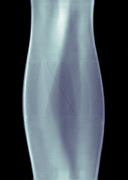
\includegraphics[width=3.420cm,height=4.800cm]{sinograms/unet2dhlcc.png}};
\end{scope}

% Network part: the bus from the input feeds the residual, the data consistency and the moment regression
\draw[decorate,decoration={brace,mirror,amplitude=6pt},thick]
    ($(menc0-west |- menc0-south)+(-0.7,-1.4)$) -- ($(mdec0-east |- menc0-south)+(0,-1.4)$)
    node[midway,below=8pt,font=\small] {U-Net $f_\theta$ (same network as UNet2D)};
\path ($(in-east)+(0.9,0)$) coordinate (b0);
\draw[bus] (b0) -- ++(0,-5.0) coordinate (b1) -| (sum-south);
\draw[bus] (b1 -| sum-south) -| (dc-south);
\node[anchor=west,align=left,font=\small] at ($(yhat-east)+(1.0,0)$) {\textbf{UNet2dHLCC}\\$\hat y$};

% Training loss (UNet2dHLCC only)
\node[draw=black!60,dashed,rounded corners=3pt,align=center,font=\small,anchor=south east] (loss)
    at ($(yhat-north)+(1.6,2.0)$)
    {\textbf{training only}: $\mathcal L=\mathrm{MSE}(\hat y,y^\star)+\alpha(t)\,(\lambda_0L_0+\lambda_1L_1)$\\
     HLCC penalty $L_n=\|(I-\Pi_{H_n})\,a^{\hat y}_n\|^2/V$, annealed by $\alpha(t)$};
\draw[bus,dashed] (yhat-north) -- (yhat-north |- loss.south);

% HLCC moment regression P_K: first row, left to right
\node[op,text width=4.8cm,anchor=north west] (my) at ($(in-west)+(-0.8,-7.0)$)
    {moments of the measured views\\
     $a^{y}_n(\theta)=\sum_s y(\theta,s)\,U_n(s/S)$\\
     $\theta\in\Theta_{\mathrm{acq}}$, $n=0,\dots,4$};
\draw[bus] (b1) -- (b1 |- my.north);
\node[op,text width=5.9cm,right=0.6cm of my] (reg)
    {harmonic regression\\ fit $\tilde a_n\in H_n$ on $\Theta_{\mathrm{acq}}$, evaluate on all views\\
     {\scriptsize $H_n=\mathrm{span}\{\cos m\theta,\sin m\theta\}_{m\le n,\ m\equiv n\,(2)}$}};
\node[op,text width=2.9cm] (myhat) at (yhat-south |- reg.center)
    {moments of $\hat y$\\ $a^{\hat y}_n(\theta)$, all the views};
\node[circle,draw=black!60,fill=\HLCCColor,inner sep=1pt,font=\small] (delta)
    at ($(reg.east)!0.5!(myhat.west)$) {$-$};
\draw[bus] (yhat-south) -- (myhat.north);
\draw[bus] (my) -- (reg);
\draw[bus] (reg) -- node[above,font=\small,opacity=1] {$\tilde a_n$} (delta);
\draw[bus] (myhat) -- node[above,font=\small,opacity=1] {$a^{\hat y}_n$} (delta);

% second row, right to left
\path (delta) ++(0,-4.1) node[op,text width=5.0cm] (corr)
    {correction of the missing views\\
     $\delta(\theta,s)=\sum_n c_n(\theta)\,W(s)\,U_n(s/S)$\\
     $W(s)=\sqrt{1-(s/S)^2}$\\ $c_n$: the corrected moments are $\tilde a_n$};
\draw[bus] (delta) -- node[right,font=\small,opacity=1] {$\Delta a_n=\tilde a_n-a^{\hat y}_n$} (corr);
\node[op,text width=4.6cm,left=0.6cm of corr] (upd)
    {$\hat y_{P_4}=\hat y+M\odot\delta$\\
     $M$: missing views inside the\\ shadow of the object\\ ($\hat y>0.03\max_s\hat y$)\\[3pt]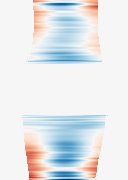
\includegraphics[height=1.9cm]{sinograms/p4_correction_2d.png}\\[-1pt]{\scriptsize $M\odot\delta$ on the test sample}};
\draw[bus] (corr) -- (upd);
\coordinate (title) at ($(my.north west)+(0,0.75)$);

\pic[shift={(0,0,0)}] at ($(upd.west)+(-2.6,0)$)
    {Box={name=yp4,
        caption={},
        xlabel={{"",}},
        zlabel={},
        fill=\IOColor,
        opacity=0.6,
        height=24.0,
        width=0.4,
        depth=17.1}};

\draw[connection] (upd.west) -- node {\midarrow} (yp4-east);

\begin{scope}[shift={(yp4-east)}]
    \node[canvas is zy plane at x=0,transform shape,inner sep=0pt] at (0,0)
        {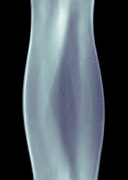
\includegraphics[width=3.420cm,height=4.800cm]{sinograms/unet2dhlcc_p4.png}};
\end{scope}

\node[below=12pt,align=center,font=\small] at (yp4-nearsoutheast) {\textbf{UNet2dHLCC\_P4 $\hat y_{P_4}$}\\$180\times128$};

\node[draw=black!50,dashed,rounded corners,inner sep=0.3cm,
    fit=(title)(my)(reg)(myhat)(corr)(upd)(yp4-farnorthwest)(yp4-nearsoutheast),
    label={[anchor=north west,font=\small\bfseries,inner sep=8pt]north west:HLCC moment regression $P_4$
    (orders $0,\dots,4$, no trainable parameter, inference only)}] {};

\end{tikzpicture}
\end{document}
